\documentclass[border=10pt]{standalone}
\usepackage{tikz}
\usetikzlibrary{arrows.meta, decorations.pathmorphing}

\begin{document}

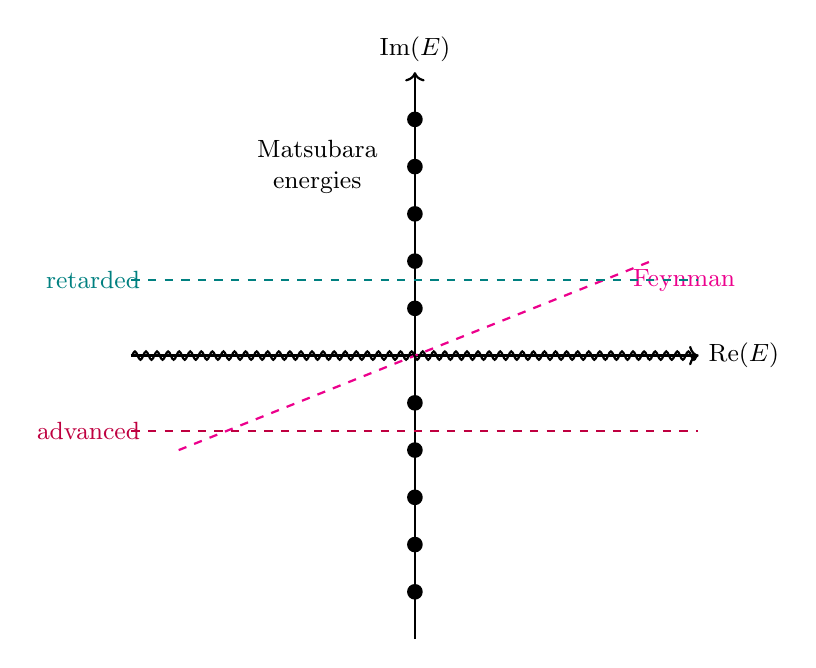
\begin{tikzpicture}[
    scale=1.2,
    every node/.style={font=\small},
    axis/.style={->, thick},
    matpoint/.style={fill, circle, inner sep=2pt},
    feynman/.style={dashed, magenta, thick},
    retarded/.style={dashed, teal, thick},
    advanced/.style={dashed, purple, thick},
    wavy/.style={decorate, decoration={snake, amplitude=1.5pt, segment length=4pt}, thick}
]

% Axes
\draw[axis] (0, -3) -- (0, 3) node[above] {$\mathrm{Im}(E)$};
\draw[axis] (-3, 0) -- (3, 0) node[right] {$\mathrm{Re}(E)$};

% Matsubara energies (discrete points on Im axis)
\foreach \y in {-2.5, -2, -1.5, -1, -0.5, 0.5, 1, 1.5, 2, 2.5} {
    \node[matpoint] at (0, \y) {};
}

% Label for Matsubara energies
\node[align=center, left=10pt] at (0, 2) {Matsubara\\energies};

% Feynman propagator (dashed magenta line with positive slope)
\draw[feynman] (-2.5, -1) -- (2.5, 1);
\node[feynman, right] at (2.2, 0.8) {Feynman};

% Retarded propagator (horizontal teal dashed line above real axis)
\draw[retarded] (-3, 0.8) -- (3, 0.8);
\node[retarded, left] at (-2.8, 0.8) {retarded};

% Advanced propagator (horizontal purple dashed line below real axis)
\draw[advanced] (-3, -0.8) -- (3, -0.8);
\node[advanced, left] at (-2.8, -0.8) {advanced};

% Wavy line along real axis
\draw[wavy] (-3, 0) -- (3, 0);

\end{tikzpicture}

\end{document}